\documentclass[12pt]{article}
\usepackage[left=2cm, top=3cm]{geometry}
\usepackage[utf8]{inputenc}
\usepackage{graphicx}
\usepackage{times}
\usepackage[czech]{babel}
\usepackage[breaklinks, unicode]{hyperref}
\hypersetup{colorlinks = true}
%\usepackage{breakurl}


\begin{document}

	\begin{titlepage}
		\begin{center}
			
\includegraphics[scale=0.15]{fit_logo.png}
			\\
			\vspace{\stretch{0.152}}
			{\Large
				 \huge{{IFJ, IAL 2020 - Dokumentace\\[0.5em]}}}
				 {\Huge\textbf{{Implementace překladače jazyka IFJ20}}}\\[0.5em]
				 \huge{Tým 48 - Varianta II}\\[0.5em]
				 \smallskip
				 \LARGE{Implementovaná rozšíření: UNARY, FUNEXP}
			\vspace{\stretch{0.218}}
			\\
		{\Large
			\begin{tabular}{l c r}           % this spacing is hideous. Completely hideous. But it works.
            \textbf{Marek Filip} \hspace{1em}(\textbf{xfilip46})\hspace{1.61em} -- 27\% \\
            Vojtěch Bůbela (xbubel08)\hspace{1.03em} -- 23\% \\
            Vojtěch Fiala \,\,\,\,\,(xfiala61)\,\,\,\,\,\,\,\,\, -- 23\% \\
            Ondřej Míchal \,\,(xmicha80)\quad -- 27\% \\
            \end{tabular}
			
		}
		\end{center}
	\end{titlepage}
    
    \tableofcontents
    
    \newpage
    \section{Úvod}
    \large{Tato dokumentace popisuje implementaci překladače imperativního jazyka IFJ20, který je založen na jazyce Go. Implementace překladače byla zadána jako projekt do předmětů IFJ a IAL.}
    \section{Práce v týmu}
    
        \subsection{Komunikace}
        
        \large{Týmová komunikace probíhala převážně osobně a nebo skrz aplikaci Discord. Náš tým měl každý týden pravidelné schůzky, na kterých jsme probírali pokrok, jakého jsme za uplynulý týden dosáhli a určovali si milníky, kterých chceme dosáhnout do další schůzky.}
        
        \subsection{Verzovací systém}
        Pro správu verzí projektu jsme použili verzovací systém git a platformu GitHub.
        
        \subsection{Rozdělení práce}
        Základní rozdělení práce na jednotlivých částech projektu proběhlo na prvním meetingu. Následně jsme si pak s jednotlivými problémy ještě navzájem vypomáhali. Konkrétní rozdělení práce popisuje následující tabulka:
        \newline
        
        \begin{center}
        \begin{tabular}{|p{11em}|p{21em}|}
            \hline
            \textbf{Marek Filip} (\textbf{xfilip46}) &  
            Organizační záležitosti, syntaktická analýza, sémantická analýza, zásobníková struktura, testování, dokumentace\\
            \hline
            Vojtěch Bůbela (xbubel08)  & Lexikální analýza, generování cílového kódu,
            testování, dokumentace\\
            \hline
            Vojtěch Fiala (xfiala61) & Lexikální analýza, generování cílového kódu, testování, dokumentace, prezentace\\
            \hline
            Ondřej Míchal (xmicha80) & Lexikální analýza, sémantická analýza, tabulka symbolů, testování, dokumentace, git podpora\\
            \hline
        \end{tabular}
        \end{center}
        Na mírně nerovnoměrném rozdělení bodů jsme se společně dohodli na základě toho, že mezi výkonností jednotlivých členů byly rozdíly a shodli jsme se, že je tímto způsobem dorovnáme.
    
    \section{Implementace jednotlivých částí projektu}
        \subsection{Lexikální analýza}
        \label{lex}
            První krok při tvorbě překladače je lexikální analýza. Pro její implementaci jsme vytvořili deterministický konečný automat založený na diagramu \ref{DKA}.
            
            Ze standardního vstupu jsou načítány jednotlivé znaky (v případě, že se jedná o bílý znak či komentář, je zahozen), které dále DKA analyzuje, přidává do struktury \verb!string! \footnote{Struktura {\texttt{string}} pochází z knihovny {\texttt{str.h}}, která je dostupná na stránkách projektu předmětu IFJ} a skládá z nich tokeny. Token je reprezentován strukturou \verb!token_t!, která se skládá z typu a atributu.
            
            Typ tokenu může být buď identifikátor, literál, datový typ, operátor a nebo spe\-ciální typ -- konec řádku, konec souboru a nebo neplatný typ. Jestliže se jedná o identifikátor, je jeho název dále porovnán s tabulkou klíčových slov a na základě výsledku tohoto srovnání se rozhodne, zda se jedná o klíčové slovo či název proměnné a nebo funkce.
            
            Atribut tokenu je tvořen datovou strukturou \verb!union! a v případě, že je typ tokenu literál, obsahuje jeho hodnotu.
            
            Výsledný token je poté předán k dalšímu zpracování.
    
    \newpage
    \section{Syntaktická analýza}
        Při návrhu jsme čerpali z populární mezinárodní knihy známé pod pseudonymem \uv{Dragon Book} \cite{DragonBookSyn}.
        Zádání nám určilo využití LL(1) gramatiky pro analýzu shora dolů a metodu precedenční tabulky pro analýzu zespodu nahoru. Jako první se sepsali pravidla LL(1) gramatiky. Pro správný postup byly použity instrukce získané z Dragon Book. Revize této gramatiky však probíhala několikrát, z důvodu neúplného pochopení zadání či špatného prvotního návrhu. 
        
        Sestavená gramatika (včetně gramatiky pro výrazy pro první nulté odevzdaní) pak byla využita pro sestavení LL tabulky. Pro sestavení tabulky jsme postupovali dle instrukcí získaných ze záznamu democvičení IFJ ze dne 18. 10. 2011. Správnost LL tabulky (pro účely implementace) jsme pak zkontrolovali pomocí webové aplikace autorů Radima Kocmana a Dušana Koláře\footnote{\url{http://www.fit.vutbr.cz/~ikocman/llkptg/}}.

        Analýza zhora dolů je pak implementována metodou rekurzivního sestupu, kde se gramatická pravidla rozvíjí dle volání jiných funkcí nebo rekurzivního volání sebe sama. Tento postup se zdál jednodušší z důvodu banální implementace a absence zásobníku. Díky rozšíření FUNEXP jsme nemuseli řešit předávání kontroly nějakým "hackem" a výsledný kód by měl proto působit \uv{čistěji}.

        Precedenční analýzu jsme započali po nultém pokusném odevzdání. V týmu jsme se dohodli na zvolení rozšíření FUNEXP a UNARY, takže se již od začátku počítalo se složitějším návrhem a následnou implementací. Rozšíření FUNEXP znamenalo hodně implementačních detailů a problému při různém stupni zanoření volání funkce a jejího správného vyhodnocení vzhledem na ostatní operátory včetně čárky, z pohledu tabulky to znamenalo přidat operátor \texttt{,}, který má nejmenší precedenci s tím, že na některých místech tabulky přibylo více "=" operátorů.
        
        Pro precedenční analýzu je použita struktura zásobníku (dále stack). Stack je implementoval obecně, díky chytrému využití maker pro abstrakci datového typu obsaženého ve stacku a díky shell skriptu generující nové soubory jsme mohli tento stack s lehkostí využít i pro potřeby sémantické analýzy a generování kódu.
        Na základu syntaktické analýzy je vybudována analýza sémantická.
        \newpage
    
    \section{Sémantická analýza}
        Implementace sémantické analýzy blízce následuje syntaktickou analýzu. V úvodní části se značným problém prokázala být kombinace analýzy zhora dolů a zdola nahoru. Důvodem byla tvrdá hranice mezi informacemi, které každá část analýzy má. 

        V rámci analýzy se ihned generuje tříadresný kód. Tento přístup byl zvolen s vidinou ulehčené práce. V průběhu implementace se ale objevila potřeba pro alespoň omezené použití abstraktního syntaktického stromu. Během analýzy se bohatě využívá několik datových struktur:

        \begin{itemize}
            \setlength\itemsep{0.05em}
            \item tabulka symbolů uživatelských funkcí
            \item tabulka symbolů interních funkcí
            \item zásobník volaných funkcí
            \item zásobník dočasných identifikátorů
            \item zásobník proměnných na levé straně přiřazení
            \item zásobník typů, které by volaná funkce měla vrátit ve výrazu
        \end{itemize}

        V rámci vyhodnocování výrazů se každý výsledek redukce uložil do dočasné proměnné. Tento přistup umožnil už
        poměrně lehké propojení obou částí analýzy (zhora dolů a zdola nahoru). Zároveň ale tento přístup přináší značnou režii.

        Rozšíření FUNEXP přineslo komplikaci ve formě nejasnosti vracených hodnot z volání funkcí. Tyto nejasnosti
        byly částečně vyřešeny sledováním "hloubky" \break zanoření ve výrazu a na základě kontextu se pro funkci určí možná vrácená hodnota. I bez rozšíření FUNEXP je ale volání funkcí v ifj20 náročnější, protože nevyžaduje, aby
        funkce před voláním byla deklarována. Proto, kromě již zmí\-něného mechanizmu, se každé funkční volání přidává
        na zásobník. Po zdánlivě úspěšném zpracování analýzy se každé funkční volání porovná s tabulkami symbolů, kde
        jsou dostupné signatury interních i uživatelských funkcí.

        Interně vyhodnocování výrazů analýza rozumí relačním operacím, ale neu\-možňuje práci s nimi mimo výrazy v
        hlavičkách prvků řídích běh programu (if, for).

        Inspirace pro sémantickou analýzu: \cite{DragonBookSem}

    
    
    \newpage
    \subsection{Generování cílového kódu}
        Generování cílového kódu IFJ20code je posledním krokem v běhu našeho překladače. Na začátku generování kódu dochází k vygenerování všech podporovaných vestavěných funkcí na začátek výstupu. Mezikód je generován na základě instrukcí v podobě tříadresného kódů, které jsou generátoru předány jako položky v lineárně vázaném seznamu. Při tvorbě struktury tříadresného kódů jsme čerpali z \cite{DragonBook}. 
        
        Argumenty tříadresného kódu jsou typově rozděleny - prefixy \verb!i,f,s,d,!\texttt{b} značí, o jaký typ argumentu se jedná (\verb!int,float,string,!\texttt{identifier,}\newline \texttt{bool}).
        Na základě těchto prefixů jsou složky tříadresného kódu zpracovány a převedeny do formátu vhodného k vygenerování instrukce.
        
        Následně se na základě jednotlivých instrukcí zí\-skaných z tříadresného kódů generuje výsledný mezikód.
    \newpage
    \section{Datové struktury}
        \subsection{Tabulka symbolů} 
            Dle zadání je implementace založena na tabulce s rozptýlenými položkami. Při implementaci se vycházelo z kódu, který byl vytvořen v rámci předmětu IJC.
            
            Implementace tabulky symbolů probíhala v čtyřech iteracích, kdy se kromě funkcionality a implementačních
            detailů řešily problémy s komplexností API. Komplexnost se ve výsledku vyřešila tak, že veřejné API je v
            souboru \break \texttt{symtable.h} a zbytek je v interní \texttt{symtable-private.h}.

            Tabulka symbolů je komplexní struktura, která funguje na několika úrovních:
            \begin{itemize}
            \setlength\itemsep{0.05em}
            \item Funkční bloky oddělují symboly v jednotlivých funkcích. Slouží také pro reprezentaci globálního rámce. Jsou
            implementovány jako jednosměrný lineá\-rní seznam. Funkční bloky obsahují identifikátor funkce, parametry,
            návrato\-vé hodnoty a zásobník rámců.

            \item Zásobník rámců je lineárním seznam, kdy nejvrchnější prvek představuje nejhlouběji zanořený rámec.
            Struktura, reprezentující rámec, obsahuje odkaz na vnější rámec a samotnou tabulku symbolů.

            \item Tabulka symbolů je tabulka s rozptýlenými položkami, která obsahuje klíče, které jsou asociovány se symboly.

            \item Symbol je struktura, představující identifikátor, který obsahuje token (viz Lexikální analýza \ref{lex}).
            \end{itemize}
            Lineární seznam byl pro většinu struktur zvolen pro lehkost implementace a níz\-kou paměťovou režií. Samotná
            hashovací tabulka je schopná se realokovat, pokud její kapacita začne být naplňována. K realokaci dojde, pokud
            lineární seznam v polích tabulky dosáhne zhruba 70\% maximální \uv{povolené}  délky.

            Po vytvoření tabulka symbolů obsahuje vždy jeden funkční blok (globální), v něm zásobník rámců a v něm jeden
            rámec.

            \newpage
        \subsection{Lineární seznam - 3AC}
            Jednosměrný lineárně vázaný seznam je implementován ve 2 souborech --\break \verb!three-address-code.c! a \verb!three-address-code.h!. Je založen na do\-mácí úloze č. 1 z předmětu IAL. Využíván je k předávání instrukcí tříadresného kódu. Skládá se z ukazatele na aktivní položku a na první položku v seznamu. Tělo jednotlivých položek obsahuje typ operandu, 3 argumenty (výsledek a 2 parametry operace) a ukazatel na další položku. Tělo tříadresného kódu je založeno na \cite{DragonBook}.

        \section{Závěr}
            Po zveřejnění zadání nás projekt zarazil svou rozsáhlostí a komplexitou. Projekt jsme vypracovávali od jeho zveřejnění, nicméně jeho kompletní dokončení se nám nepodařilo. Jednotlivé části jsme testovali za pomoci knihovny gtest\footnote{\url{https://github.com/google/googletest}} a větší celky pak za pomoci end-to-end testů a knihovny  bats\footnote{\url{https://github.com/bats-core/bats-core}}. Při řešení projektu jsme využili znalosti získané na přednáškách předmětů IFJ a IAL, pro některé z nás to byla také první zkušenost s větším projektem. Jako tým jsme byli dohodnutí již předem, tedy k žádným problémům nedocházelo. Při řešení projektu se projevily rozdíly ve schopnostech jednotlivých členů týmu a tyto rozdíly jsme se tedy rozhodli kompenzovat úpravou finálního rozdělení.
    
    \newpage
\bibliographystyle{czechiso}
\renewcommand{\refname}{\section{Literatura}}
\bibliography{main}
\newpage
    \begin{figure}
    \section{Příloha -- Deterministický konečný automat pro lexikální analýzu}
        \begin{center}
            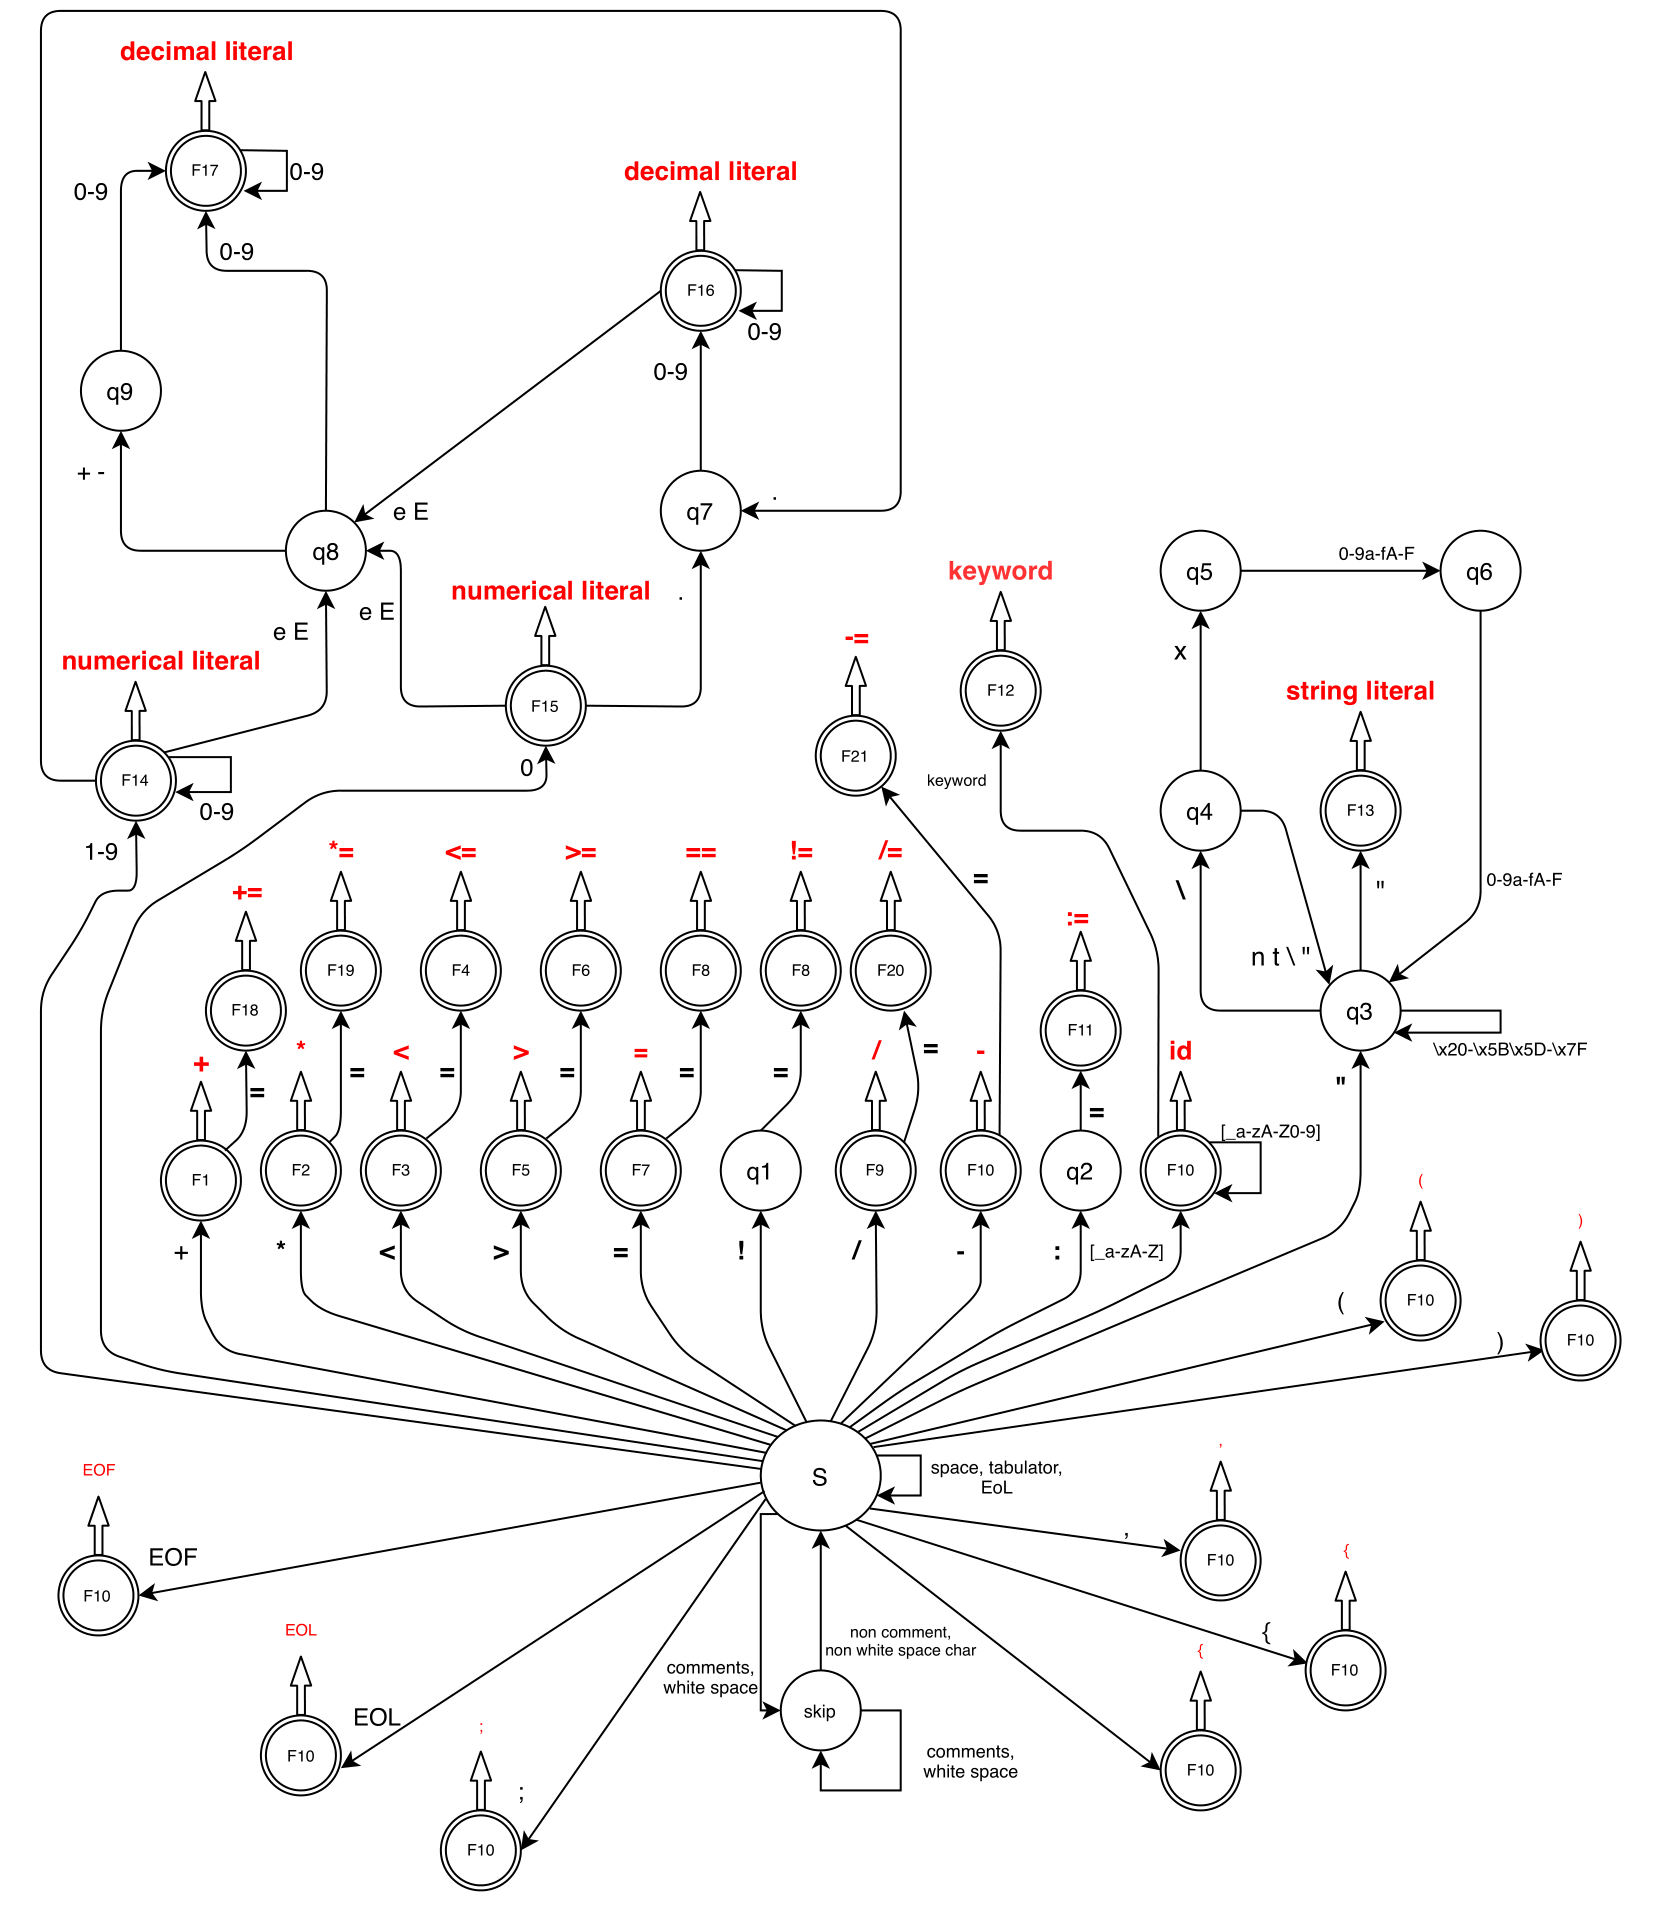
\includegraphics[scale=0.26]{scannerDKAfinalversion1.0-1.png}
            \caption{Deterministický konečný automat}
            \label{DKA}
        \end{center}
    \end{figure}
    \newpage
    \begin{figure}
    \section{Příloha -- LL gramatika}
    \begin{center}
            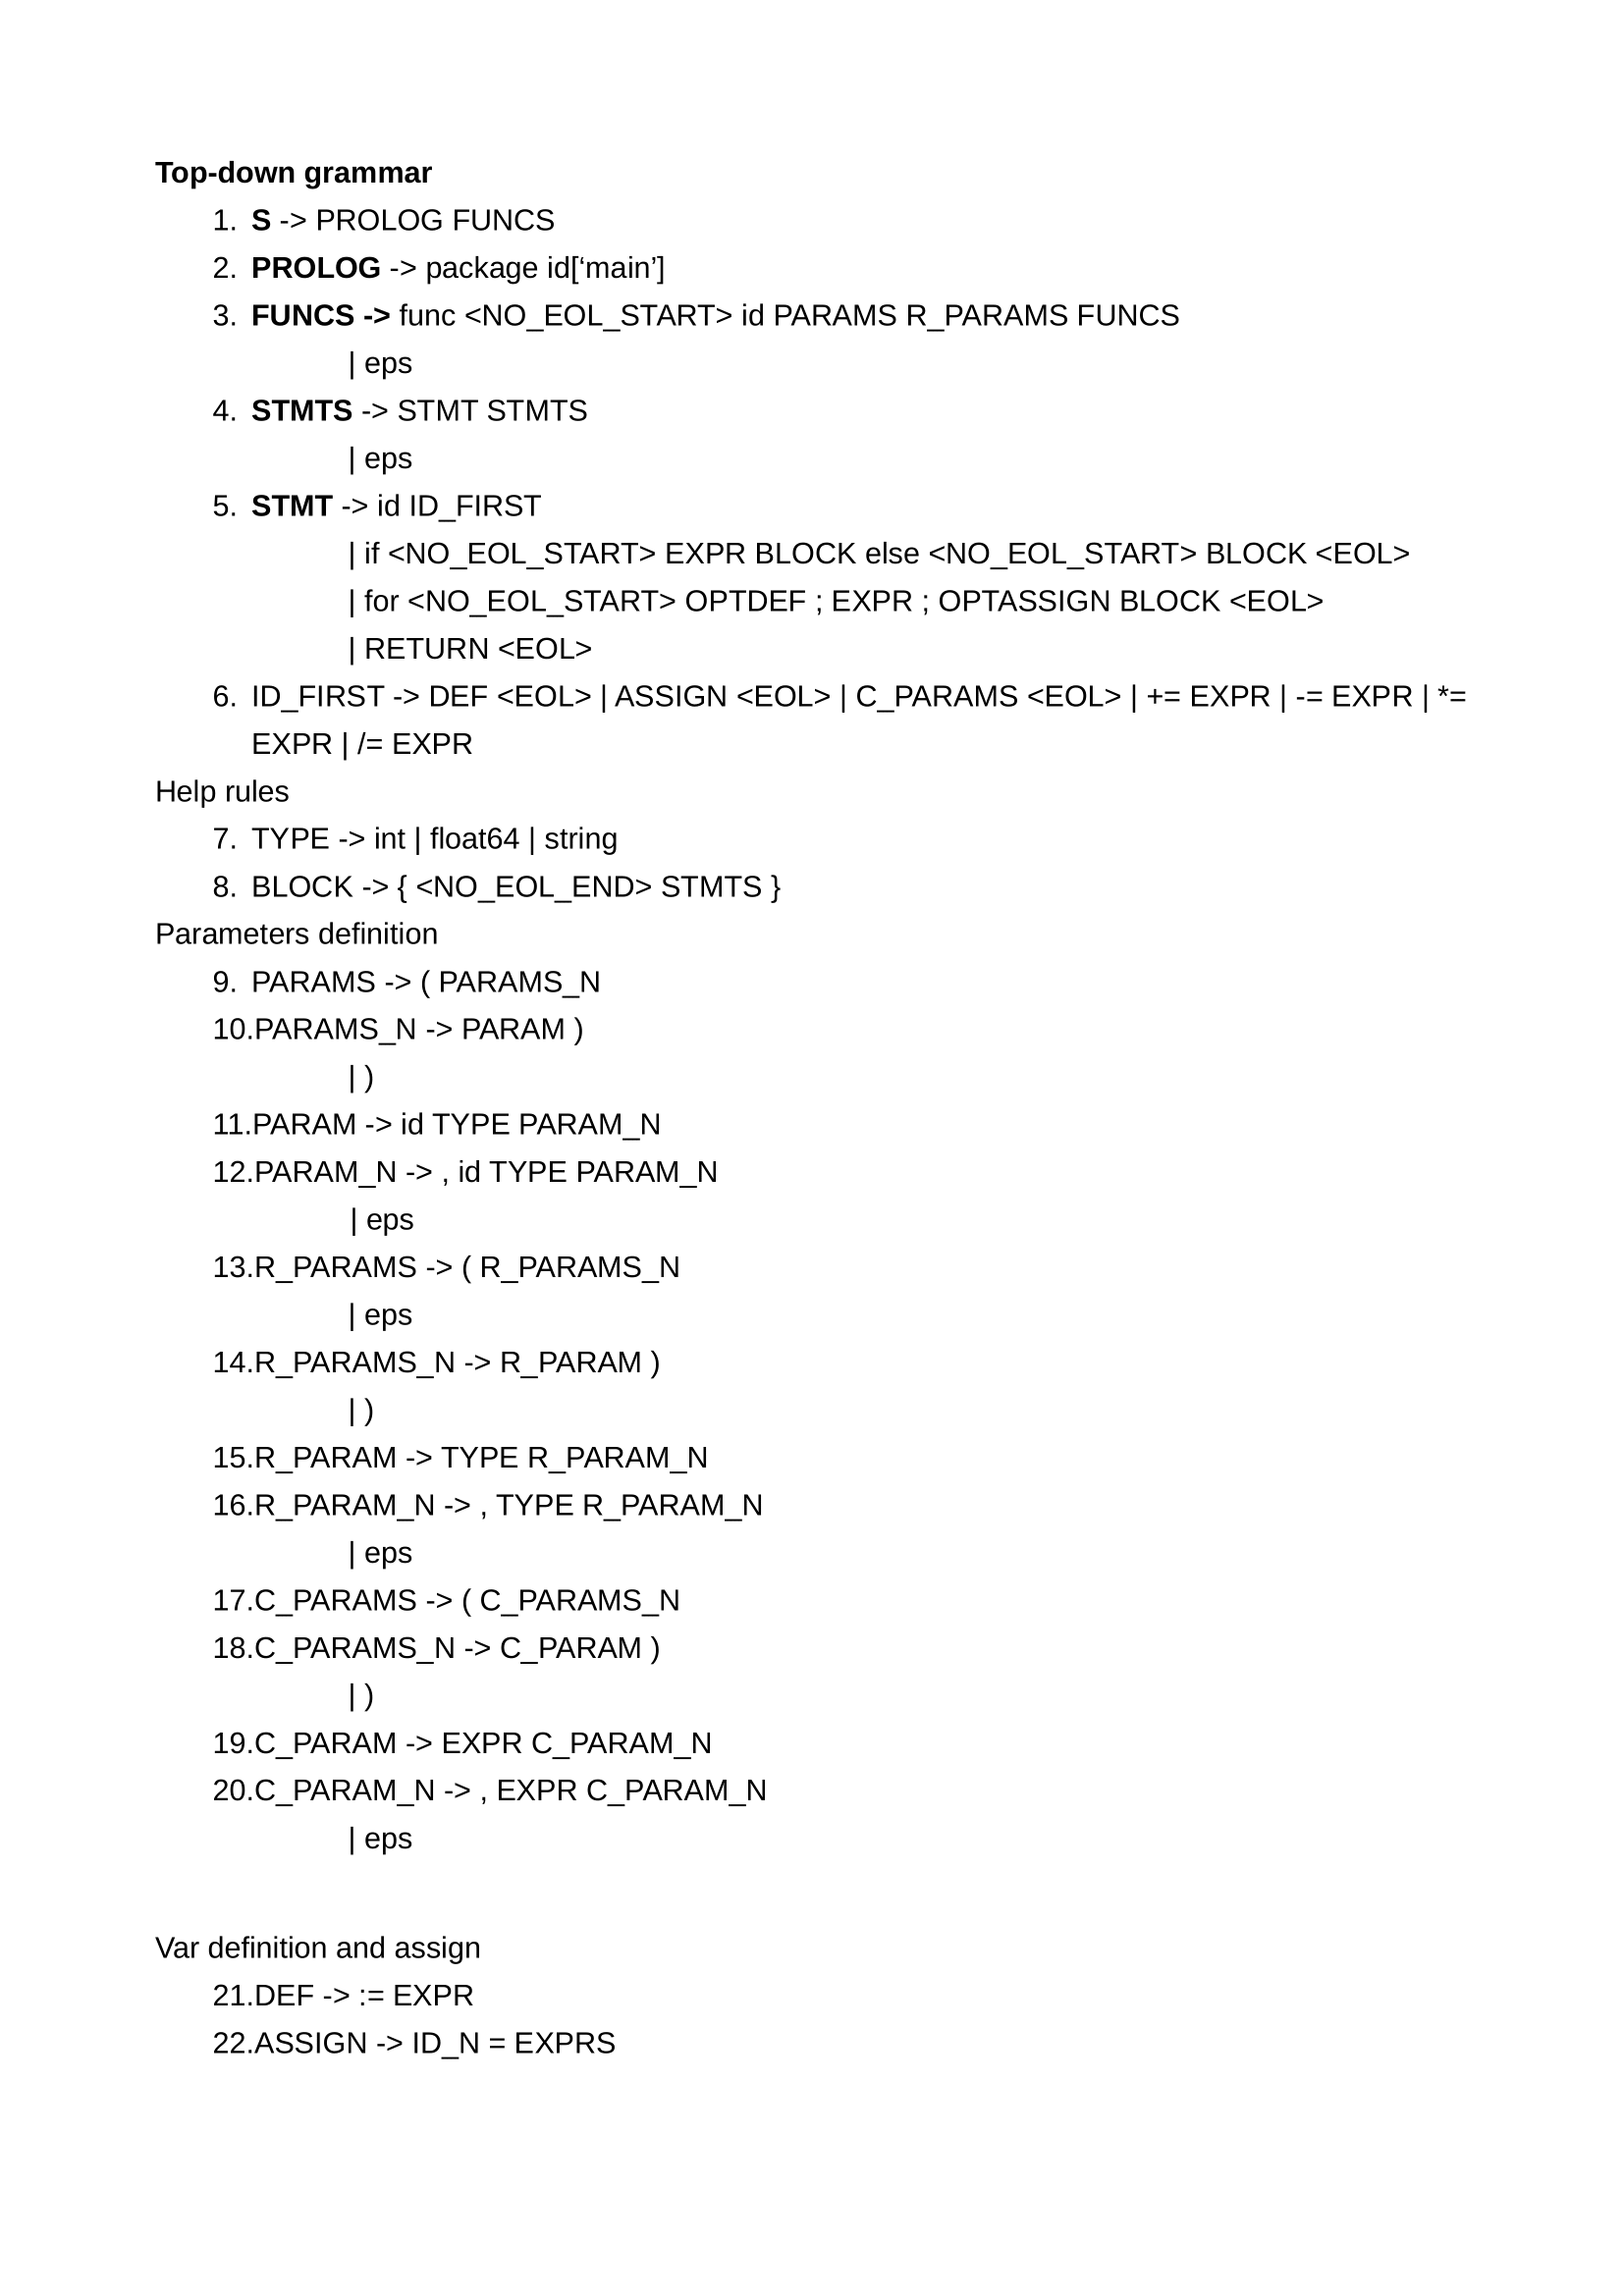
\includegraphics[scale=0.24]{grammar-1.png}
        \end{center}
    \end{figure}
    \begin{figure}
    \begin{center}
     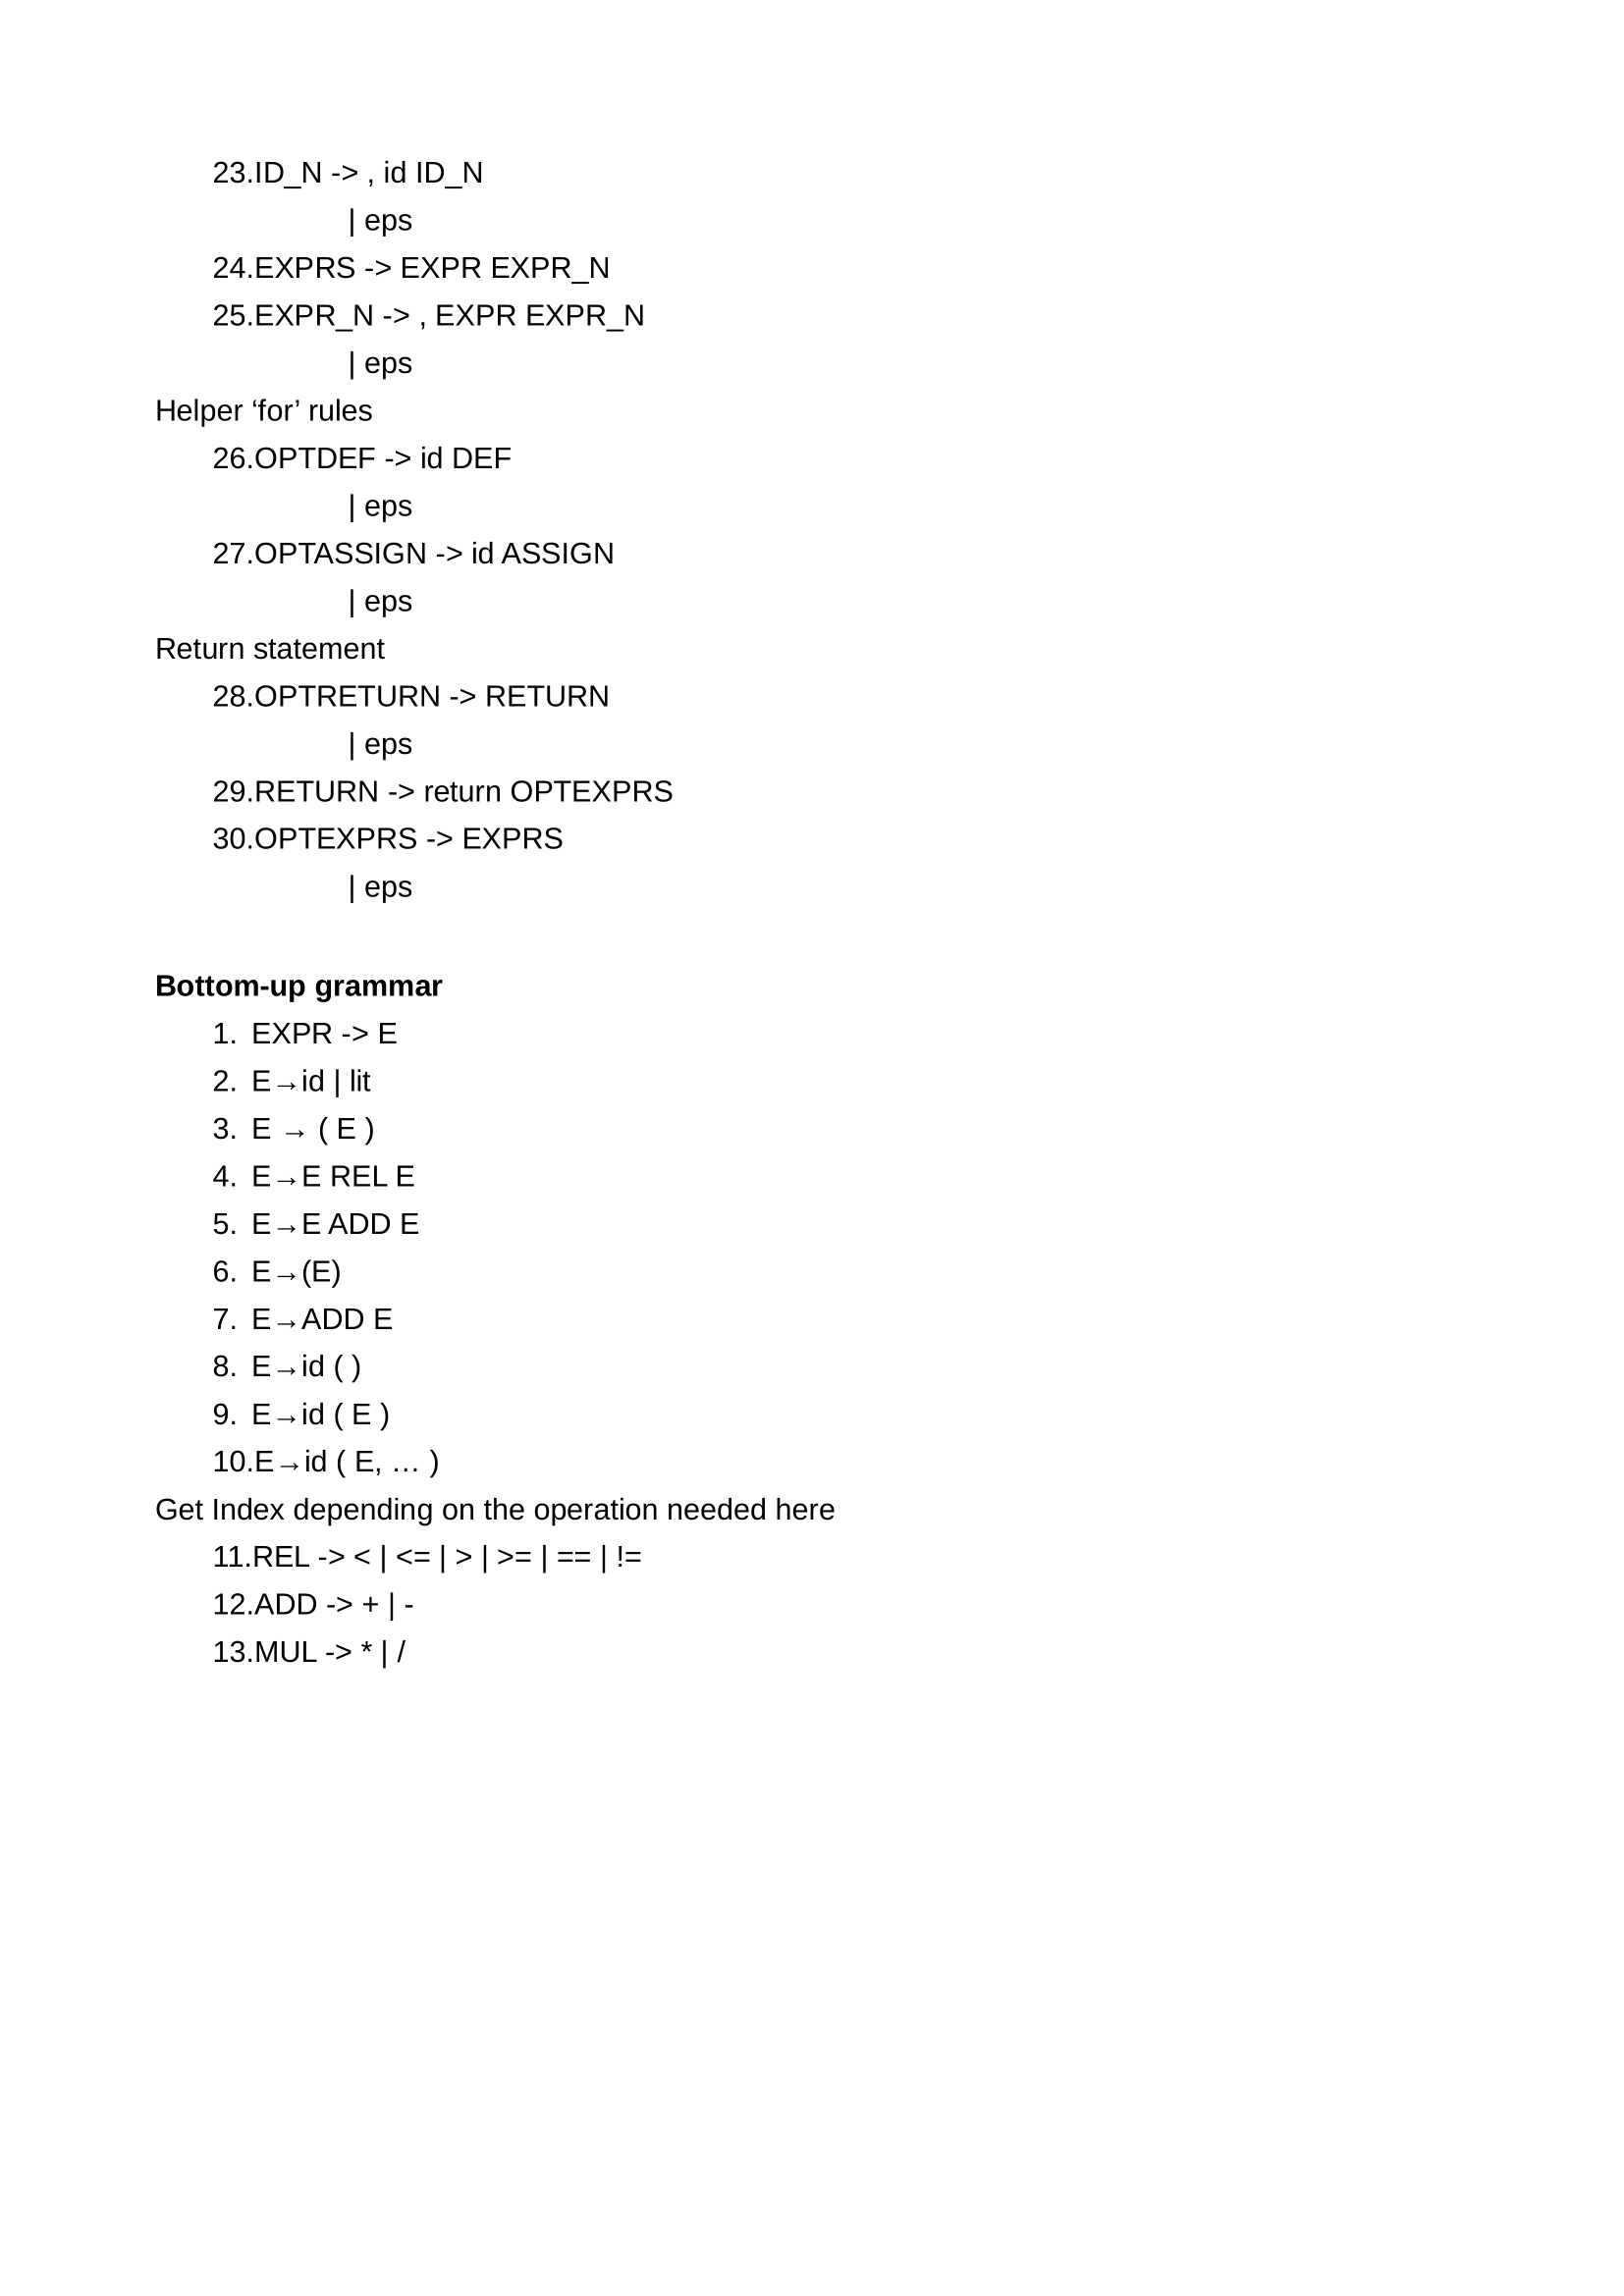
\includegraphics[scale=0.24]{grammar-2.png}
     \end{center}
     \end{figure}
    \newpage
    \begin{figure}
    \section{Příloha -- LL tabulka}
        \begin{center}
            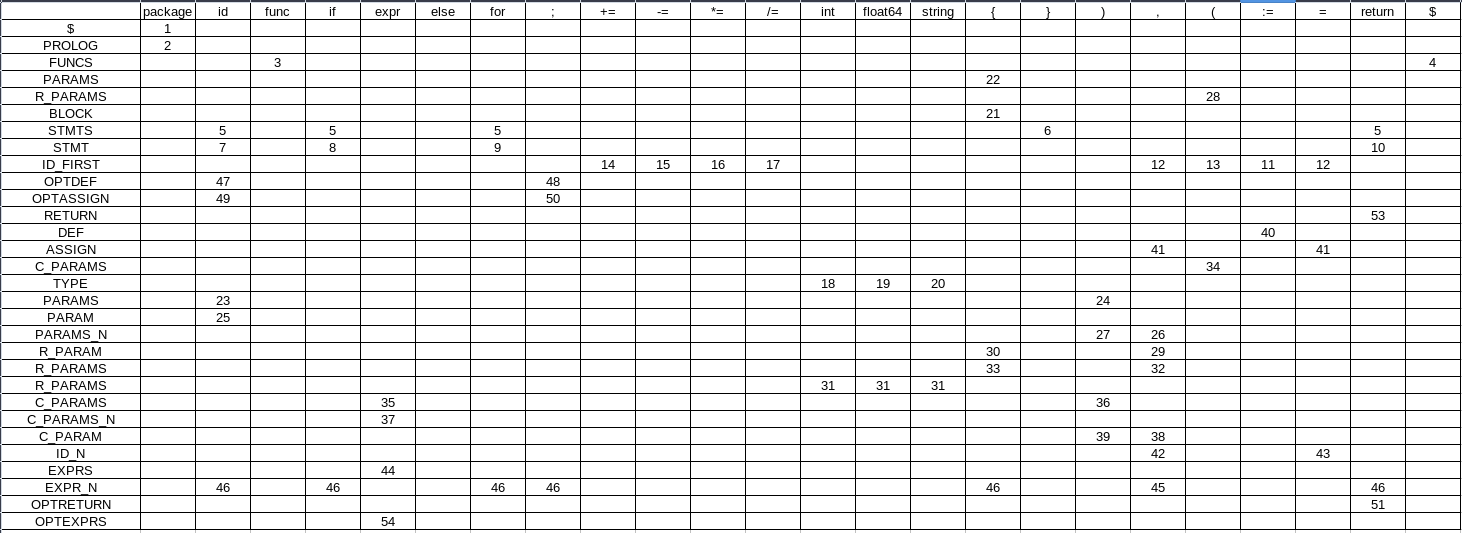
\includegraphics[scale=0.36]{unknown.png}
            \label{LLt}
        \end{center}
    \end{figure}
    \newpage
    \begin{figure}
    \section{Příloha -- Precedenční tabulka}
        \begin{center}
            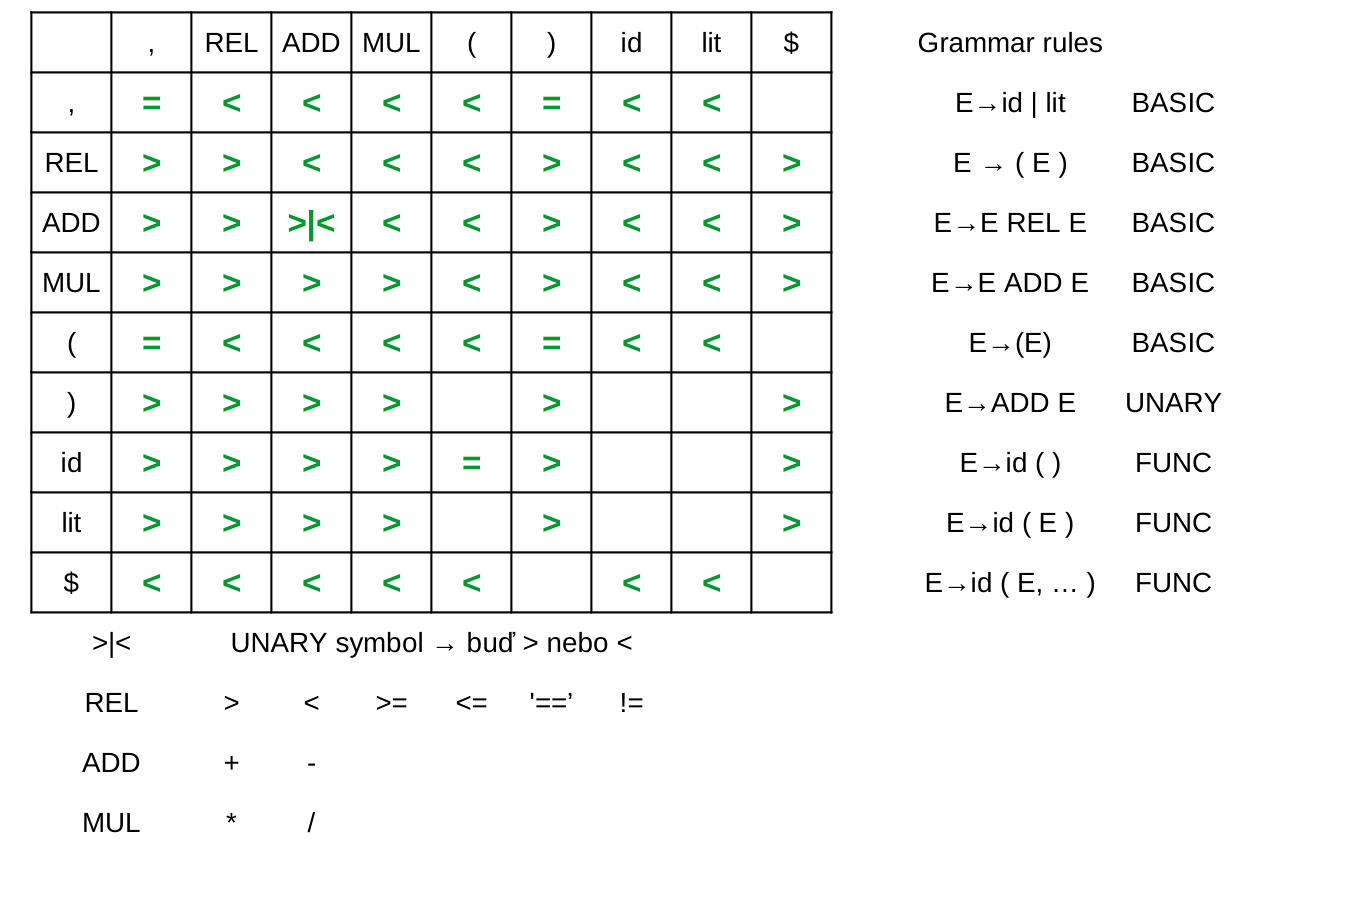
\includegraphics[scale=0.34]{precedence-table-1.png}
            \label{Prec}
        \end{center}
    \end{figure}
\end{document}
